
System wizyjny u ssaków jest dużo bardziej skomplikowany, w porównaniu do przetwarzania obrazów zestawem iloczynów skalarnych.
Neurobiolodzy nie są nawet blisko zrozumienia wszystkich operacji,
oczywiste jest, że zwykłe algorytmy informatyczne używane do rozpoznawania obrazów nie są w stanie odwzorować układu wzrokowego.
Wejściem obrazu jest oczywiście oko. 
Receptory siatkówki z tyłu gałki są nierównomiernie rozłożone i wrażliwe są na różne niesione informacje.
Inne są wrażliwe na ruch, kolor, nasycenie. Jednocześnie jednak są ze sobą powiązane.
Kiedy receptor dostaje odpowiednią informację, zmienia zachowanie innych, otaczających receptorów.
Operacje matematyczne są więc przeprowadzone jeszcze zanim obraz opuści oko.


Oko dodatkowo dostaje informacje zwrotne. 
Ludzie nie patrzą w jeden punkt, zbieramy informację zgodnie z kontekstem całego obrazu.
Dodatkowo, to sprzężenie zwrotne oddziałowuje na wyjście z receptorów.

Gdy informacje obrazu opuszczają oko, trafiają do kory wzrokowej.
Tutaj obraz jest analizowany przez mózg.
Badania nad korą wzrokową kota i świnki morskiej są podstawą modeli użytych w tym rozdziale.
Chociaż te modele są dużym krokiem w stronę symulowania systemu wizyjnego ssaków,
to wciąz jest to bardzo uproszczony model, bardzo skomplikowanego systemu.
Intensywne badania trwają by móc całkowicie zrozumieć cały proces.
Obecnie, algorytmy wypadają diametralnie słabo w porównaniu z rozpoznawaniem obrazu u człowieka.
Powód jest oczywisty, są one bardzo proste w porównaiu z rzeczywistym biologicznym systemem.

Emulowanie pewnych systemów biologicznych jest konieczne, by zwiększyć zaawansowanie systemów komputerowych.
Jednym z ważnych krokół jest zamodelowanie procesów przeprowadzanych w korze wzrokowej.
Zaczynają być zrozumiałe, jednak wciąż istnieją debaty na ich temat.
Procesy te są bardzo potężne i zrozumienie ich może prowadzić do powstania nowych narzędzi służących do rozpoznawania obrazów.

\subsection{Kora wzrokowa}
W podrozdziale będzie rozważana teoria i aplikacja dwóch modelu korowych:
\begin{itemize}
	\item PCNN (pulse coupled neural network) - Model sieci impulsowych
	\item ICM (intersecting cortical model)
\end{itemize}

Modele te są oparte na biologicznych modelach kory wzrokowej.
Jest więc konieczne, by zrobić przegląd algorytmów, 
które mocno wpłynęły na opracowanie modeli PCNN i ICM

Niezależnie od stopnia odwzorowania, czy podobieństwa do biologicznego modelu,
algorytmy użyte jako modele korowe są przydatne.
\begin{figure}[H]
 
	\centering
	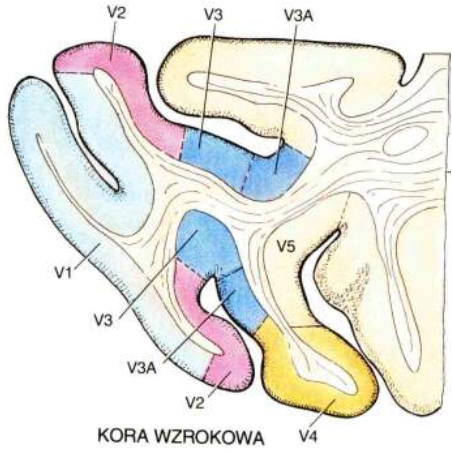
\includegraphics[width=\textwidth/2]{KoraWzrokowa.png}
	\caption{Kora wzrokowa} \label{fig:Korawzrokowa}
\end{figure} 
\begin{figure}[ht]
	\centering
	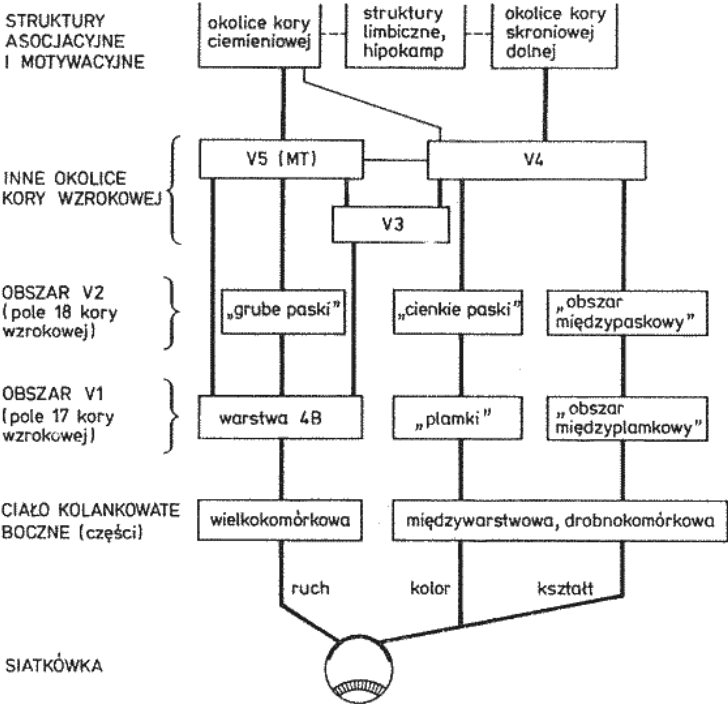
\includegraphics[width=\textwidth*4/5]{ModelKory.png}
	\caption{Model systemu wizyjnego} \label{fig:Modelkory}
\end{figure}
\ref{fig:Korawzrokowa} przedstawia korę wzrokową, a \ref{fig:Modelkory} model systemu. Istnieją dwa w znacznej mierze rozdzielone szlaki przetwarzania informacji wzrokowej, biegnącej już od oka:
\begin{itemize}
\item Wielkoziarniste komórki $PA$ siatkówki, 3 typy stożków fotorecepcyjnych, duże pola recepcyjne, szybko przewodzące aksony, pobudzenie dla światła w szerokim paśmie.
\item Drobnoziarniste komórki $PB$, 1 lub 2 typy stożków fotorecepcyjnych, małe pola recepcyjne, wolno przewodzące aksony, rozpoznają opozycje barw.
\end{itemize}
\textbf{Szlak wielkokomórkowy}: biegnie do dwóch wielkokomórkowych warstw LGN (jest w nich ok. 100.000 komórek), charakteryzuje go niska rozdzielczość przestrzenna, wysoka wrażliwość na kontrast, szybkie przesyłanie sygnałów, bez informacji o kolorze.
Ta informacja trafia przez płat potyliczny szlakiem grzebietowym do kory ciemieniowej.
Dochodzi do warstwy 4B w V1, stąd do grubych ciemnych pasków obszaru V2, analizuje informację o ruchu obiektu.
\begin{itemize}
\item W V1, warstwa $4B => V5$, lokalizacja w polu widzenia, ruch.
V5 pobudza płat ciemieniowy, PPC (tylna kora ciemieniowa), obszar 7 i 5; umożliwia to orientację przestrzenną, postrzeganie głębi i ruchu, połączenie z wzgórkami czworaczymi (orientacja oczu).
\end{itemize}
\textbf{Szlak drobnokomórkowy} ma 4 drobnoziarniste warstwy i 10 razy więcej komórek niż wielkokomórkowy w LGN.
Duża rozdzielczość przestrzenna, kolor, wolniejszy przesył informacji, niska wrażliwość na kontrast.
Ta informacja trafia szlakiem brzusznym do kory dolnoskroniowej.
\begin{itemize}
\item $V1 => V2$ obszar międzyplamkowy, reaguje na orientację linii, daje dużą ostrość widzenia, bez koloru.
\item $V1 => V3$ obszar plamkowy, reaguje na kształty, reakcja na kolor w neuronach w ciemnych prążkach V3.
\item $V2 => V4$, główny obszar analizy koloru, informacja dochodzi do kory dolnoskroniowej (IT).
Obszar IT w płacie dolnoskroniowym ma neurony reagujące na złożone obiekty. 
\end{itemize}



\subsection{Model Hodgkina-Huxleya}
Badania na temat kory wzrokowej ssaków przedstawione ponad pół wieku w pracy Hodgkina i Huxleya
zdefiniowały system opisujący potencjał błonowy następująco:
$$I=m^3 hG_{Na} (E-E_{Na}) + n^4G_K(E-E_K)+G_L(E-E_L) $$
\begin{itemize}
\item $I$ -- prąd jonowy
\item $m$ -- prawdopodobieństwo otwarcia kanału
\item $G$ -- konduktancja (dla sodu, potasu i przenikania)
\item $E$ -- Potencjał
\end{itemize}
Prawdopodobieństwo pisane następująco:
$$\frac{dm}{dt}=a_m(1-m)-b_mm$$
$a_m$ jest współczynnikiem bramek nie otwartych, a $b_m$ jest współczynnikiem aktywacji bramek.

Ważność korowego systemu jest taka, że neurony są opisane jako równanie różniczkowe.
Prąd jest zależny od współczynników zmian poszczególnych chemicznych elementów.
Dynamika neuronu jest opisana jako proces oscylacyjny.
\subsection{Model Fitzhugh-Nagumo}
Zachowanie neurona w pracy popełnionej przez Fitzhugh i Nagumo kilka lat później, 
zostało opisane jako oscylator van der Pola.
Ten model jest opisany w różnoraki sposób, ale częścią wspólną zawsze jest sparowany oscylator dla każdego neuronu.
W swojej pracy podają przykład, gdzie $x$ jest pobudzeniem, a $y$ przywróceniem. 
$$\varepsilon\frac{dx}{dt}=-y-g(x)+I$$
$$\frac{dy}{dt}=x-by,$$

Gdzie:
\begin{itemize}
\item $g(x) = x (x-a) (x-1)$
\item $0<a<1$ 
\item $I$ jest prądem wejściowym 
\item $\varepsilon\ll1$
\end{itemize}
\ref{fig:FitzhughNagumoequation} ukazuje system oscylacyjny opisany równaniami Fitzhugh-Nagumo.
Te równania opisują prosty system i bardzo proste sumulacje potrafią zaprezentować różne charakterystyki systemu.
Dla przypadku $\varepsilon=0.3$, $a=0.3$, $b=0.3$ i $I=1$ można uzyskać zachowanie jak na rysunku \ref{fig:FitzhughNagumoequation}.
Po zmianie wartości $b=0.6$ można wygenerować system przedstawiony na rysunku \ref{fig:FitzhughNagumoequation2}.
Model zaprezentowany przez Fitzhugh i Nagumo jest ważny z tego względu,
że opisuje neurony w taki sposób, który może zostać użyty w wielu różnych biologicznych modelach.
Każdy neuron reprezentuje dwa oscylatore połączone z innymi neuronami.
\begin{figure}[ht]
	\centering
	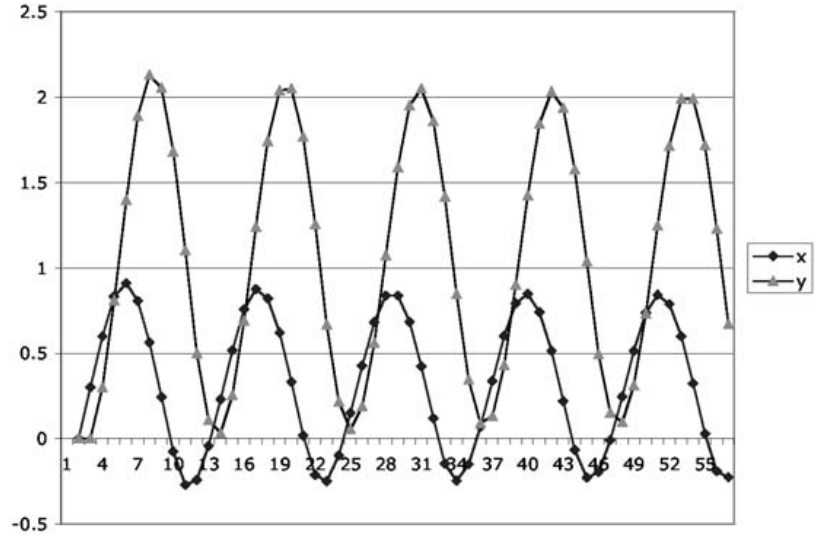
\includegraphics[width=\textwidth*4/5]{FitzhughNagumoequation.png}
	\caption{System oscylacyjny opisany równaniami Fitzhugh-Nagumo} \label{fig:FitzhughNagumoequation}
\end{figure}
\begin{figure}[ht]
	\centering
	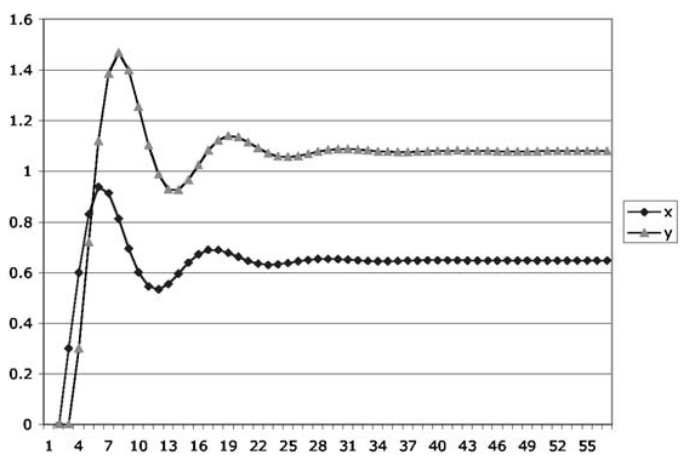
\includegraphics[width=\textwidth*4/5]{FitzhughNagumoequation2.png}
	\caption{System oscylacyjny opisany równaniami Fitzhugh-Nagumo} \label{fig:FitzhughNagumoequation2}
\end{figure}
\subsection{Model Eckhorna}
\begin{figure}[H]
	\centering
	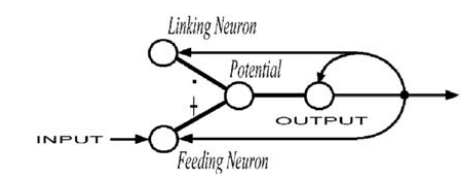
\includegraphics[width=\textwidth*3/5]{../EckhornNeuron.png}
	\caption{Neuron typu Eckhorna } \label{fig:EckhornNeuron}
\end{figure}

Eckhorn wprowadził model oprarty na korze wzrokowej kota.
Jego schemat przedstawiony na rysunku \ref{fig:EckhornNeuron}.
Komunikacja pomiędzy neuronami została pokazana na rysunku \ref{fig:PCNNNeuron}.
Sieć składa się z warstwy neuronów połączonych ze sobą dwoma rodzajami sprzężeń zwrotnych:
\begin{itemize}
\item feeding(F)
\item linking (L)
\end{itemize}
Rezultatem porównania jest napięcie membrany, $U_m$, które jest następnie porównane do lokalnego progu, $\Phi$

Model Eckhorna prezentują następujące równania:
$$U_{m,k} (t)=F_k(t)[1+L_k (t)]$$
$$F_k(t)=\sum\limits_{i=1}^N [\omega_{ki}^f Y_i(t)+S_k(t)+N_k(t)]\bigotimes I (V^a, \tau^a,t)$$
$$L_k(t)=\sum\limits_{i=1}^N [\omega_{ki}^l Y_i(t)+N_k(t)]\bigotimes I (V^l, \tau^l,t)$$
$$ \mathbf{Y_k(t)} =
\left\{ \begin{array}{ll}
1 & \textrm{dla $U_{m,k}(t)\geq \phi_k(t)$}\\ 
0 & \textrm{pozostałe przypadki}
\end{array} \right.$$

W przypadku ogólnym
$$X(t)=Z(t)\bigotimes I(v,\tau,t)$$

da się przedstawić jako:
$$X[n] = X[n-1]e^{\frac{-t}{\tau}} + V Z[n] $$

$N$ jest liczbą neuronów, $\omega$ wagą synaptyczną, $Y$ wyjściem binarnym, $S$ pobudzeniem zewnętrznym.
Typowe zakresy wartości wynoszą $\tau^a=[10,15]$, $\tau^l=[0.1, 1.0]$, $\tau_s=[5,7]$, 
$V^a=0.5$, $V^l=[5,30]$, $V^s=[50,70]$, $\phi_o=[0.5,1.8]$.

\begin{figure}[ht]
	\centering
	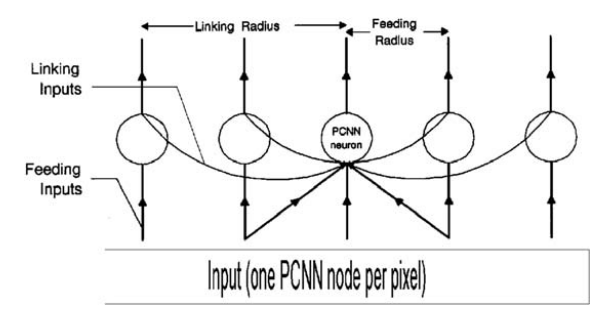
\includegraphics[width=\textwidth*4/5]{../PCNN.png}
	\caption{Neuron PCNN} \label{fig:PCNNNeuron}
\end{figure}
\subsection{Model Rybaka}
Elementem badań Rybaka była kora wzrokowa świnki morskiej i odkrył podobne zależności, co w modelu Eckhorna.
Równania są różne, natomiast samo zachowanie neuronu jest całkiem podobne.
Neuron Rybaka ma 2 porównania $X$ i $Z$. 
Następuje ich interakcja z pobudzeniem, $S$ : 
$$X_{ij}^S=F^S\bigotimes||S_{ij}||$$
$$X_{ij}^I=F^I\bigotimes||Z_{ij}||$$
$$Z_{ij}=f\left\{\sum X_{ij}^S - \left( \frac{1}{\tau p+1} \right) X_{ij}^I -h \right\}$$

Gdzie $F^S$ są połączeniami centrum/otoczenie.
$F^I$ to lokalne połączenia kierunkowe, $\tau$ to stała czasowa i $h$ jest globalnym inhibitorem.
$f{}$ jest funkcją progowania.
\subsection{Model Parodi}
Wciąż istnieje małe podobieństwo do rzeczywistego modelu kory wzrokowej.
Parodi zaproponował alternatywę dla modelu Eckhorna. 
Argumentami przeciwko modelowi Eckhorna były m.in. brak synchronizacji w neuronach,
nieporządane podobne wyjścia dla elementów poruszających się i stacjonarnych, 
czy to, że modulacje neuronu w sprzężeniu L były znacznie wyższe niż przewidywał to model Eckhorna.

Parodi zaproponował więc model alternatywny, zawierając w nim opóźnenia związane z połączeniami synaptycznymi
i wprowadził reset neuronu \textit{en masse}.
$$\frac{\partial V(x,y,t)}{\partial t} = - \frac{V(x,y,t)}{\tau} 
+ D\Delta ^2V(x,y,u)+h(x,y,t)$$

$V_i$ jest potencjałem $i$--tego neuronu, $D$ jest dyfuzją $(D = \frac{a^2}{C} R_c)$,
$R_c$ jest rezystancją sprzężeniową neuronu, $t= C R_l$, $R_1$ jest rezystancją upływową.
$R_c^-1<R_l^-1$

$$h_i(t)=\sum\limits_j \omega_{ij} \delta (t-t_j^s - \tau_{ij})$$
\subsection{Podsumowanie}
Biologiczne modele kory wzrokowej przedstawiają każdy neuron jako parę oscylatorów połączonych z innymi neuronami.
To różni się znacząco od tradycyjnego cyfrowego przetwarzania obrazów opartych głównie o operacje matematyczne pierwszego rzędu.
Stworzenie odpowiednio potężnych algorytmów będzie wymagało w przyszłości użycia odpowiednio potężnych maszyn.
Możliwe, że w przyszłości modele oparte o korę wzrokową ssaków będą zaimplementowane w przetwarzaniu obrazów.
